\section{Quantum Bit}

Ein klassisches Bit ist wie ein Quantum Bit (kurz: Qubit) ein Teil eines physikalischen Systems. Physikalische Qubits können auf verschiedene Weisen realisiert werden, beispielsweise durch ein zwei-Level-Atom oder Elektronenspins (Steane, 1998, Vgl. S. 22). In dieser Arbeit werden Qubits und alle weiteren Quantenkomponenten ausschließlich mathematisch interpretiert, um die Theoriegrundlagen hardwareunabhängig betrachten zu können. \newline

Ebenso befinden sich beide Bitarten nach dem Messen entweder in dem Zustand 1 oder 0. Klassische Bits können nur diese Zustände annehmen, sowohl vor dem Messen als auch danach, während Qubits vor dem Messen die Zustände \(\Ket{0}\) und \(\Ket{1}\) als orthonormale Basis für die Bildung von Linearkombinationen verwenden können.

\[\Ket{1} = \begin{bmatrix} 0 \\ 1 \end{bmatrix}, \quad \Ket{0} = \begin{bmatrix} 1 \\ 0 \end{bmatrix}\]

Linearkombinationen aus \(\Ket{0}\) und \(\Ket{1}\) werden auch als \textit{Superposition} bezeichnet. Hierfür wird der Quanten-Zustand eines Qubits als ein komplexer zweidimensionaler Vektorraum betrachtet. Solche Zustände werden wie in der Quantenmechanik mit der \textit{bra-ket} Notation, also '\(\bra{bra}\)' für Zeilenvektoren und '\(\Ket{ket}\)' für Spaltenvektoren, geschrieben.
\begin{equation} \begin{gathered}
        Statevector = \Ket{\psi} = \alpha \Ket{0} + \beta  \Ket{1} \\
        \alpha,\beta \in \mathbb{C}
    \end{gathered} \end{equation}


Dies ermöglicht häufig keine genaue Untersuchung des Quanten-Zustands, also von den Amplituden \(\alpha\) und \(\beta\). Während klassische Bits zu jeder Zeit überprüft werden können, in welchem Zustand sie sich befinden, ist bei Qubits eine genaue Überprüfung schwierig, da eine Messung ihren Quanten Zustand kollabieren lässt. \glqqWenn wir ein Qubit messen, erhalten wir entweder das Ergebnis 0, mit der Wahrscheinlichkeit \(|\alpha|^2\), oder das Ergebnis 1, mit der Wahrscheinlichkeit \(|\beta|^2\). Natürlich ist \(|\alpha|^2 + |\beta|^2 = 1\), da sich die Wahrscheinlichkeiten zu eins summieren müssen.\grqq (Nielsen und Chuang, 2001, S. 13) \newline


Das bedeutet, dass die Wahrscheinlichkeit einer Messung des Qubits \(\psi\) in dem Zustand \(x\) resultiert,

\begin{equation} \begin{gathered}
        p(\ket{x}) = | \braket{x | \psi}
    \end{gathered} \end{equation}

ist. So hat ein Qubit mit dem Statevector \( \Ket{+} = \frac{1}{\sqrt{2}} \Ket{0} + \frac{1}{\sqrt{2}}  \Ket{1}\) eine 50% Chance, nach dem Messen in den Zustand \(\Ket{0}\) zu zerfallen und somit den Wert 0 zurückzugeben, da 

\begin{align*}
    \braket{0 | +}       & = \frac{1}{\sqrt{2}}  \braket{0 |0} + \frac{1}{\sqrt{2}}  \braket{0 | 1} \\
    \braket{0 | +}       & = \frac{1}{\sqrt{2}} \cdot 1 + \frac{1}{\sqrt{2}} \cdot 0                \\
    \braket{0 | +}       & = \frac{1}{\sqrt{2}}                                                     \\
    \\
    | \braket{0 | +} |^2 & = \frac{1}{2},
\end{align*}

oder kurz gesagt, weil \(|\frac{1}{\sqrt{2}}|^2 = 0.5\) ist. Die Wahrscheinlichkeit für eine Messung des Werts 1 und dem folgenden Zerfall in den Zustand \(\Ket{1}\)  liegt bei \(\Ket{+}\) ebenfalls bei 50%. 

\newline
\newline
\exercise[type=multipleChoice]{
    \question{Frage: Was ist die Wahrscheinlichkeit, dass eine Messung des Zustands \( \Ket{-} = \frac{1}{\sqrt{2}} \Ket{0} - \frac{1}{\sqrt{2}}  \Ket{1}\) in Zustand \(\Ket{1}\) resultiert?}
    \possibleAnswers{
        \item 1) Die Wahrscheinlichkeit beträgt ebenfalls 50%.
        \item 2) Durch das negative Vorzeichen von \(\beta\) ist der Zustand ungültig.
        \item 3) Die Wahrscheinlichkeit beträgt 0%.
        \item 4) Die Wahrscheinlichkeit beträgt 100%.
    }
    \result{1}
}


\newline \newline


\subsection{Visualisierung eines Qubit Zustands}
\newline
\includeHTML{content/blochsphere.html}
\includeScript[name=blochsphere-new]{content/blochsphere-new.js}

Der Zustand eines Qubits kann auch geometrisch repräsentiert werden. Durch die Einführung einer Messung des relativen Phasenunterschieds zwischen \(\Ket{0}\) und \(\Ket{1}\) wird \textit{Formel 1} wie folgt erweitert und \(\alpha\) und \(\beta\) auf rationale Zahlen beschränkt:
\begin{equation} \begin{gathered}
        \Ket{q} = \alpha \Ket{0} + e^{i\phi} \beta  \Ket{1} \\
        \alpha, \beta, \phi \in \mathbb{R}.
    \end{gathered} \end{equation}

Wendet man zusätzlich die trigonometrische Identität \(sin^2x + cos^2x = 1\) auf den normalisierten Qubit Zustand \(|\alpha|^2 + |\beta|^2 = 1\) an, so können Alpha und Beta auch als \(\alpha = cos\frac{\theta}{2}\) und \(\beta = sin\frac{\theta}{2}\) beschrieben werden. Dies ermöglicht die Visualisierung eines Qubit Zustands als Punkt auf einer dreidimensionalen Sphäre durch die Variablen \(\theta\) und \(\psi\):
\begin{equation} \begin{gathered}
        \Ket{q} = cos\frac{\theta}{2} \Ket{0} + e^{i\phi} sin\frac{\theta}{2}  \Ket{1} \\
        \theta, \psi \in \mathbb{R}.
    \end{gathered} \end{equation}

Diese Sphäre wird \textbf{Bloch Sphere} genannt. Sie beschreibt den Zustand eines einzelnen Qubits und wird oft für die Visualisierung der Auswirkungen, die bestimmte Operationen auf ein Qubit haben, verwendet.



\begin{figure}
    \centering
    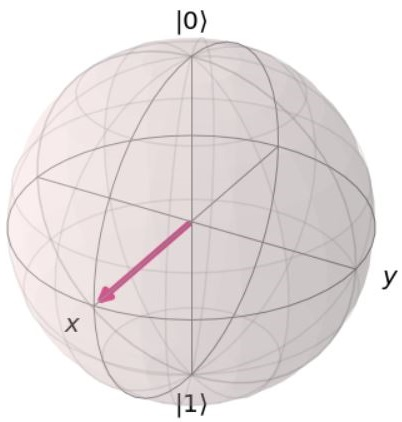
\includegraphics[width=20]{content/bloch_plus.jpg}
    \caption{Eine Bloch Sphere eines Qubits im Zustand \(\Ket{+}\), die mit dem Qiskit SDK erstellt wurde.}
    \label{fig:blochPlus}
\end{figure}





Theoretisch lassen sich durch die unendlich große Anzahl an Punkten auf der Oberfläche der Sphere auch unendlich viele Quantenzustände bilden. \glqqDiese Schlussfolgerung ist aber irreführend [...], da  die Messung eines Qubits dessen Zustand ändert, indem es aus seiner Superposition von \(\Ket{0}\) und \(\Ket{1}\) in den spezifischen Zustand kollabiert, der mit dem Messergebnis übereinstimmt. Wenn zum Beispiel die Messung von \(\Ket{+}\) den Wert 0 ergibt, dann wird der Zustand des Qubits nach der Messung \(\Ket{0}\) sein. Warum kommt es zu dieser Art von Zusammenbruch? Das weiß keiner.\grqq (Nielsen und Chuang, 2001, S. 15) \newline


Dieses Problem wird in den Hintergrund gerückt, indem Qubits so selten wie nur möglich gemessen werden. Denn auch wenn die versteckten Quantum Informationen eines Qubits nicht wirklich messbar sind, ist es möglich, sich diese Informationen zunutze zu machen. Das Verständnis jener Quantum Informationen schafft die Grundlage für Quantum Computing. \newline \newline

\exercise[type=multipleChoice]{
    \question{Frage: Wieso werden Qubits so selten wie möglich gemessen?}
    \possibleAnswers{
        \item 1) Die Messung von Qubits ist teuer, deshalb sollen Kosten gespart werden.
        \item 2) Da Messungen ungenau sind, würden viele hintereinander das Ergebnis verfälschen.
        \item 3) Nach einer Messung ist die Anzahl der möglichen Zustände eines Qubits nur noch zwei.
    }
    \result{3}
}
\newline \newline
\subsection{Zusammenspiel mehrerer Qubits}
\newline
Jedes Qubit besitzt zwei komplexe Amplituden \(\alpha\) und \(\beta\). Um den gemeinsamen Zustand von zwei Qubits zu beschreiben, werden folglich vier komplexe Amplituden benötigt. Diese werden in einem 4D-Vektor zusammengefasst:

\begin{equation}
    \Ket{\alpha} = \alpha_{00} \Ket{00} + \alpha_{01}  \Ket{01} + \alpha_{10}  \Ket{10} + \alpha_{11}  \Ket{11} = \begin{bmatrix} \alpha_{00} \\ \alpha_{01} \\ \alpha_{10} \\ \alpha_{11} \\  \end{bmatrix}
\end{equation}

Die Regeln für die Messung und Normalisierung verändern sich dabei nicht:

\[p(\ket{00}) = | \braket{00 | \alpha} |^2 = |a_{00}|^2, \]
da
\[|a_{00}|^2 + |a_{01}|^2 + |a_{10}|^2 + |a_{11}|^2 = 1. \]

Bei zwei getrennten Qubits werden beide Qubit Zustände durch ein Tensorprodukt zusammengefasst:

\begin{equation} \begin{gathered}
        \Ket{a} = \begin{bmatrix} a_0 \\ a_1 \end{bmatrix}, \quad \Ket{b} = \begin{bmatrix} b_0 \\ b_1 \end{bmatrix}
        \\
        \\
        \Ket{ba} = \Ket{b} \otimes \Ket{a} =
        \begin{bmatrix}
            b_0 \times \begin{bmatrix}a_0\\a_1\end{bmatrix} \\ \\
            b_1 \times \begin{bmatrix}a_0\\a_1\end{bmatrix}
        \end{bmatrix}
        = \begin{bmatrix}b_0 a_0\\b_0 a_1\\b_1 a_0\\b_1 a_1\end{bmatrix}
    \end{gathered} \end{equation}

Diese Zusammenfassung der Zustände mittels dem Tensorprodukt lässt sich auf eine beliebige Anzahl an Qubits anwenden. Hierbei gilt allerdings:

\glqqWenn wir \(n\) Qubits haben, müssen wir den Überblick über \(2^n\) komplexe Amplituden behalten. Wie wir sehen können, wächst die Größe der Vektoren exponentiell mit der Anzahl der Qubits. Dies ist der Grund, warum Quantencomputer mit einer großen Anzahl von Qubits so schwer zu simulieren sind. Ein moderner Laptop kann problemlos einen allgemeinen Quantenzustand von etwa 20 Qubits simulieren, aber die Simulation von 100 Qubits ist zu schwierig für die größten Supercomputer.\grqq (ANIS u. a., 2021, Textbook ’Multiple Qubits and Entangled States’ - Chapter 1)


\newline  \newline
\subsection{Entangled States}
\newline

Befindet sich ein einzelnes Qubit in einer Superposition, so zerfällt diese nach einer Messung in die Zustände \(\Ket{0}\) oder \(\Ket{1}\). Wenn das Qubit aber Teil eines Systems \(\Ket{s}\) aus mehreren Qubits ist, wie zum Beispiel bei dem \textit{Bell State}, dann hat die Messung von Qubit \(A\) eine direkte Auswirkung auf den Zustand von Qubit \(B\) und lässt dessen Superposition ebenfalls zerfallen.

\begin{equation}
    \Ket{s} = \frac{1}{\sqrt{2}} (\Ket{00} + \Ket{11})
\end{equation}
Dieser zwei-Qubit-Zustand \textit{Bell State} befindet sich in einer Superposition und kann nach einer Messung ausschließlich in \(\Ket{00}\) oder \(\Ket{11}\) zerfallen. Wird nur ein Qubit des \textit{Bell States} gemessen, ist sofort klar, in welchen Zustand sich das andere Qubit befinden muss. Erhält man nach der Messung von Qubit \(A\) zum Beispiel den Wert 1, so verändert sich der gemeinsame Zustand zu \(\Ket{s} = \Ket{11}\). \newline
Hierbei ist es egal, wie physisch weit entfernt Qubit \(A\) von Qubit \(B\) ist, da sie \textit{entangled} sind. Dieses Phänomen wird auch als \textit{Quantum Nonlocality} bezeichnet.


\newline \newline
\exercise[type=multipleChoice]{
    \question{Frage: Wann hat die Messung eines Qubits Auswirkungen auf die Messung eines anderen Qubits?}
    \possibleAnswers{
        \item 1) Wenn sie miteinander verschränkt sind.
        \item 2) Gar nicht. Die Messung eines Qubits ist unabhängig von anderen Qubits.
        \item 3) Sobald ein Qubit gemessen wurde, denn danach haben alle anderen Qubits im System denselben Zustand.
    }
    \result{1}
}





\newline \newline

\subsection{Quellen}
[ANIS u. a. 2021] Qiskit: An Open-source Framework for Quantum Computing. 2021\newline
[Nielsen und Chuang 2001] Nielsen, Michael A. ; Chuang, Isaac L.: Quantum computation and quantum information. In: Phys. Today 54 (2001), Nr. 2, S. 60\newline